
%(BEGIN_QUESTION)
% Copyright 2013, Tony R. Kuphaldt, released under the Creative Commons Attribution License (v 1.0)
% This means you may do almost anything with this work of mine, so long as you give me proper credit

Calculate the input voltage ($V_{in}$) to this opamp circuit, given the current and resistor values shown.  Assume the opamp is capable of ``rail-to-rail'' output voltage swings, and that the arrow points in the direction of {\it conventional} flow.  Be sure to denote whether the input voltage is a positive or a negative value (with reference to ground):

$$\includegraphics[width=15.5cm]{i01953x01.eps}$$

$V_{in}$ = 

\underbar{file i01953}
%(END_QUESTION)





%(BEGIN_ANSWER)

$V_{in}$ = -2.86 V

%(END_ANSWER)





%(BEGIN_NOTES)

{\bf This question is intended for exams only and not worksheets!}.

%(END_NOTES)

